%&latex
\documentclass{amsart}
\usepackage{graphicx}

\begin{document}

%+Title
\title{An explanation of simulating PDMP grain boundary coarsening}
\author{Joe Klobusicky}
\maketitle
%-Title


%-Abstract



\section{Initial conditions}
We start with a list of $N$ grains 
\begin{equation}
(g_1,\dots, g_N) = ((a_1,s_1), \dots, (a_N,s_N)),
\end{equation} 
where grain $g_i$ has area $a_i$ and $s_i$ sides.  Since we are working with a trivalent network, we have the conservation of polyhedral defect as our (only) initial condition
\begin{equation}
\sum s_i-6 = 0.
\end{equation}
Note that we have no constraints on area.  

\section{Area advection and critical events: no side flipping}
Each grain $g_i$ grows at rate $s_i-6$, so that in the absence of any random changes,
\begin{equation} 
a_i(t) = a_i(0)+(s_i-6)t
\end{equation}
When a grain reaches zero area, it is deleted from the list.  Grain deletion triggers side numbers of grains to change randomly, depending on the number of sides of the deleted grain.  The basic rules are:\begin{enumerate}
\item If a two sided grain deletes, two grains are randomly selected to lose two sides.
\item If a three sided grain deletes, two grains are randomly selected to lose one side.
\item If a four sided grain deletes, two grains are randomly selected to lose one side.
\item If a five sided grain deletes, two grains are randomly selected to lose one side, and one grain is randomly selected to gain one side.
\end{enumerate}

To randomly select which grains change sides, we select a grain proportional to the number of sides that grain possesses.  Thus, we first select that a grain with $k$ sides will delete, with a probability 
\begin{equation}
p_k = \frac{kN_k}{\sum_{j=2}^M jN_j}.
\end{equation}
$N_j$ is the number of grains with $j$ sides.  After this, we select among $k$ sided grains with equal probability.  

This description is actually a little off, since we cannot allow for grains to have less than two sides, or more than $M$ sides.  Thus, for 2-gon (2 sided grain) deletion, $k$-gon probabilities $p_k^2$ are given by
\begin{equation}
p_k^2 = \frac{kN_k}{\sum_{j=4}^M jN_j},\quad k = 4,\dots, M 
\end{equation}

Similarly, we have
\begin{equation}
p_k^3 = \frac{kN_k}{\sum_{j=3}^M jN_j}, \quad k = 3,\dots, M 
\end{equation}

\begin{equation}
p_k^4 = \frac{kN_k}{\sum_{j=3}^M jN_j}, \quad k = 3,\dots, M 
\end{equation}
\begin{equation}
p_k^3 = \frac{kN_k}{\sum_{j=3}^{M-1} jN_j}, \quad k = 3,\dots, M-1 .
\end{equation}

Thus, in the absence of side deletion, grains change their areas with respect to the $n-6$ rule at a constant rate until a grain deletes.  Grains are then selected to change sides according to $k$-gon probabilities, and begin drifting again.

\section{Side flipping}
The model allows for us to have a flipping parameter $\beta$ based on the number of particles in the system.  Thus, we imagine that each particle has a $\beta$ clock, and one such clock ringing denotes a side deletion. Side deletion corresponds to two grains randomly gaining a side, and two grains randomly gaining a side, with flipping probabilities
\begin{equation}
p_k^{side} = \frac{kN_k}{\sum_{j=3}^{M-1} jN_j}, \quad k = 3,\dots, M-1 .
\end{equation}


 Given a state $(g_1,\dots,g_N)$, if no flips occur, we then know the exact time until a grain deletes:
\begin{equation}
T = \min_{s_i<6} \frac {a_i}{6-s_i}. 
\end{equation}
Since each grain has a Poisson clock of intensity $\beta$, the random variable of the first clock to ring, denoted $Y$,  is also Poisson, with intensity $N\beta$.  Thus the procedure for including side flipping is as follows:\begin{enumerate}
\item Draw from $Y \sim Poisson(N\beta)$.
\item If $Y<T$, evolve grains for time $Y$, change sides according to side deletion rules and probabilities, and return to step 1.
\item If $Y>T$, evolve grains for time $T$, change sides according to grain deletion rules and probabilities, and return to step 1.
\end{enumerate}

\section{Simulations thus far}
So far I've shown the following, where I've let the maximum number of sides $M= 20$ with initial distribution of 9,000 $n$-gons, $n= 2, \dots, 10$, with initial areas for each $n$-gon distributed uniformly between 0 and 1. I've added the extra 10 possible side classes because I didn't want buildup to occur at $M$-gons, which happens for high $\beta$ since flipping allows grains to transfer from $M-1$ sides to $M$ sides, but not from $M$ sides to $M-1$ sides.
\subsection{Coarsening rates}
The graph of the average grain area becomes linear as $\beta \rightarrow 0$, and is convex as $\beta$ increases.  This is true not only for average area of the entire network, but also restricting on $n$-gons, $n= 2, \dots, M$.  Also of note is the average area of each $n$-gon is increasing.
 \begin{figure}
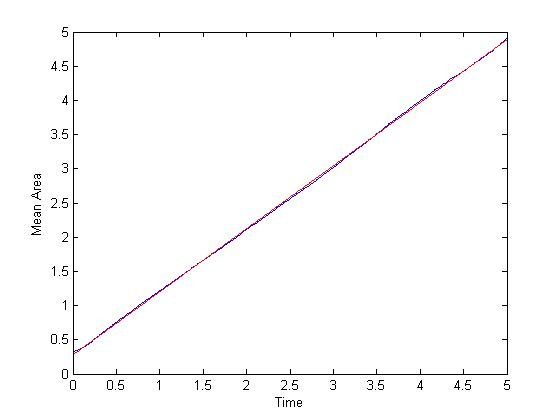
\includegraphics{meanregareazero.jpg}
\caption{\textbf{Mean area of grains with $\beta = .01$} Mean area is plotted with line of best fit $y_1 = .2806+.9214x$  (the lines are indistinguishable). The correlation between average area and $y_1$ is $r^2= .9998$. }\label{av1}
\end{figure}

\begin{figure}
\begin{centering}
\includegraphics[width=.5\textwidth]{averageareas.jpg}
\caption{Average areas of grains with sides 2-10 at $\beta= 0$.  Note how for each collection of $n$-gons,for $n= 2, \dots, M$, average area increases linearly.  Similar behavior holds for $\beta= .1$ and $\beta= 1.$}\label{averagewhole}
\end{centering}
\end{figure}
\subsection{$n$-gon fraction distribution}
The discrete denisites which plot the fraction of $n$-gons, $n = 1, \dots, M$, become stationary as $\beta \rightarrow 0$.  As $\beta$ increases, densities diffuse and become more uniform as time increases. 

\begin{figure}
        \begin{centering}
        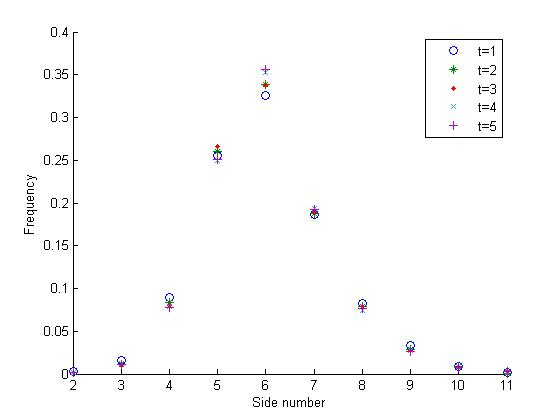
\includegraphics[width=.5\textwidth]{classdistzero.jpg}
        \caption{Frequency of side number for $\beta= .01$ for various times.}\label{sidedist1}
\end{centering}
\end{figure}

\subsection{$n$-gon densities}
Densities for $n$-gons, $n = 1, \dots, M$,  tend to increase in mean and variance as time increases. There appears to be a nonzero mode for densities with greater than six sides, but no such mode for densities with less than six sides.
\begin{figure}
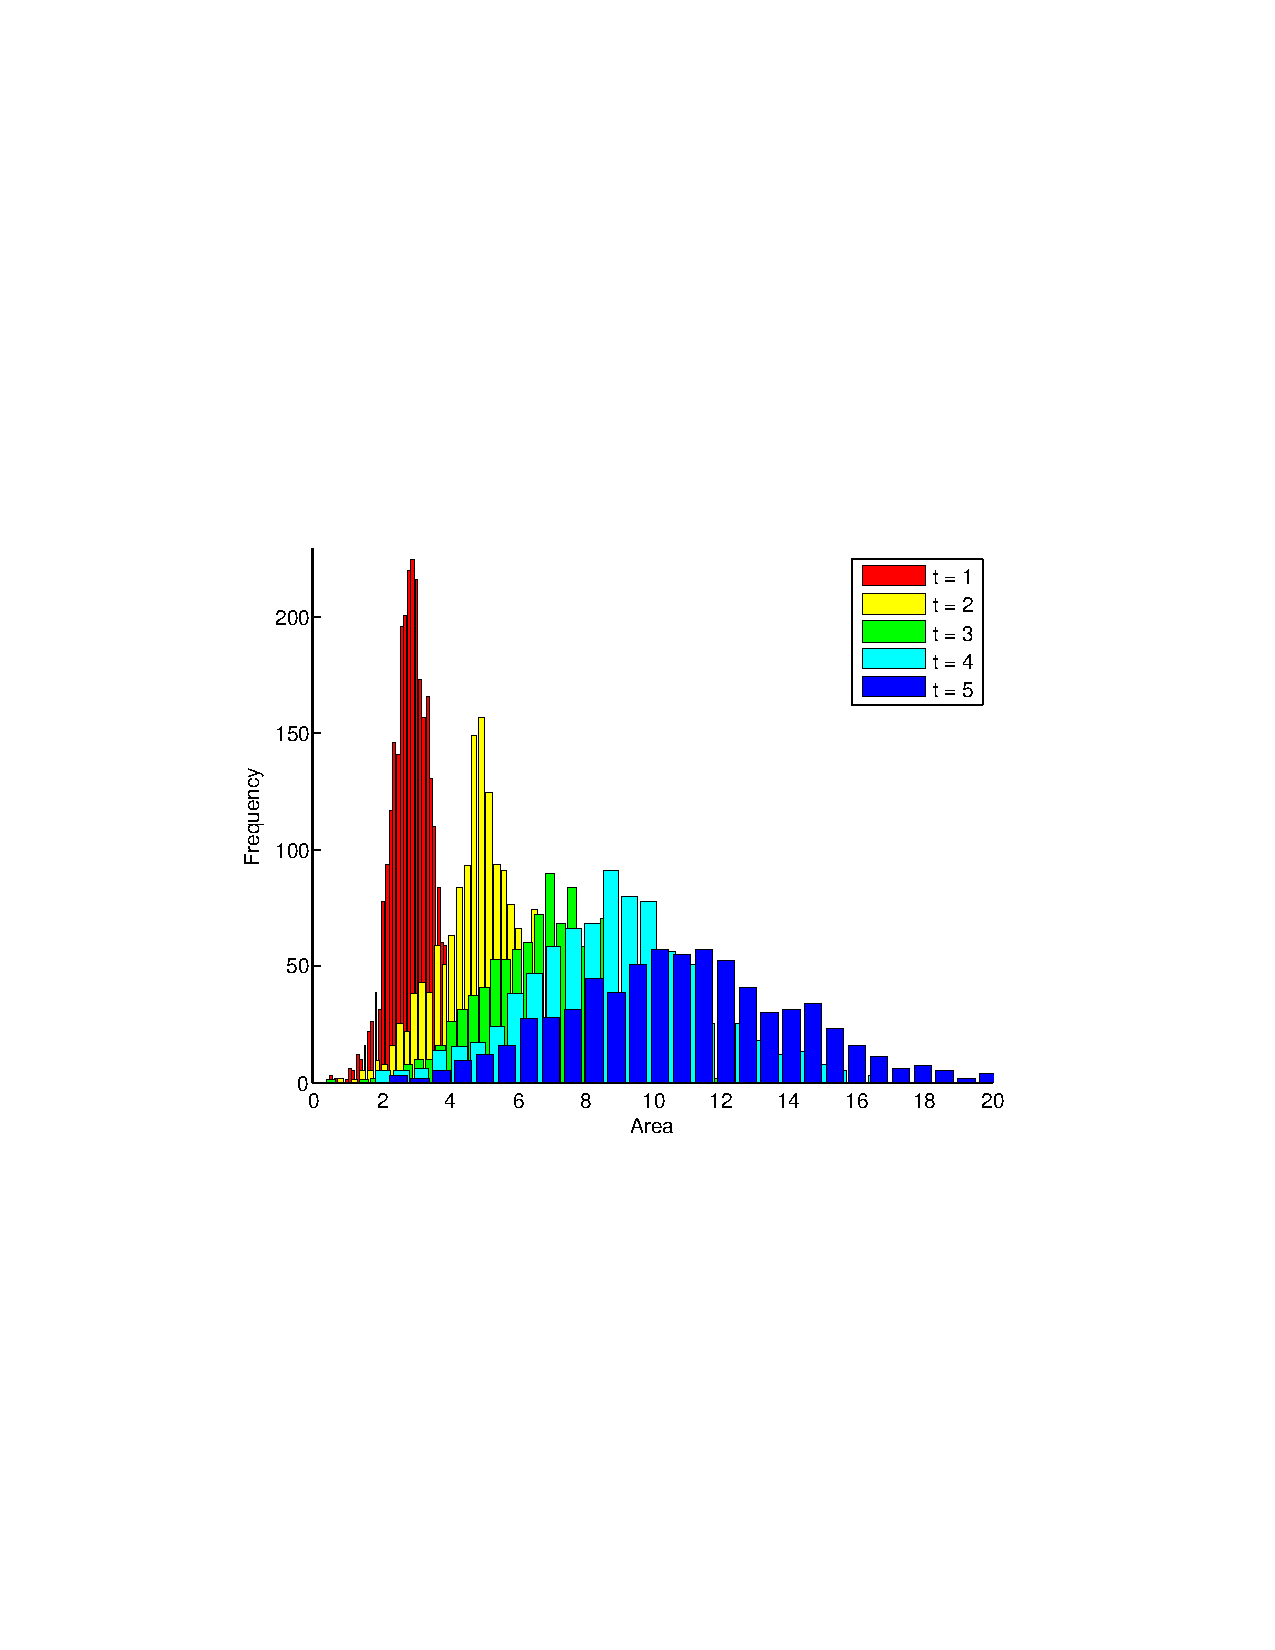
\includegraphics[width=\textwidth]{histbetazerotier8.pdf}
\vspace{-130pt}
\caption{Histograms of eight-sided grain densities at $\beta = .01$.}
\end{figure}

\subsection{Side to grain deletion rates}
Ratios of total side to grain deletions appear to grow at a log-like rate.  This differs from the Fradkov model, which assumes a constant ratio in their  formulation of kinetic equations for grain area densities.
 \begin{figure}
        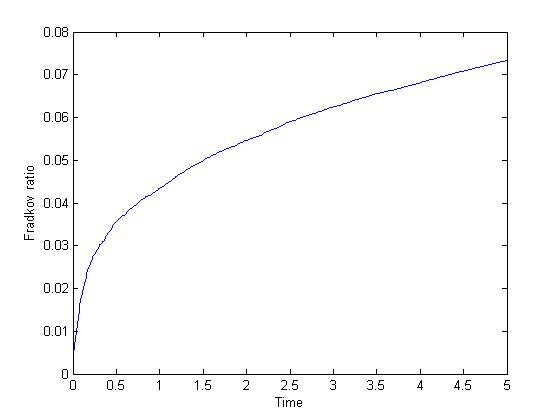
\includegraphics[width=.5\textwidth]{coarseratiobetatenth.jpg}
        \caption{Side to grain deletion ratio $\gamma_\beta(t)$ at $\beta=.1$.}
 \end{figure}       
        

\section{Things to do}

\begin{enumerate}
\item  First and foremost, get the code running for $>10^6$ grains.  As of now, we only have simulations on $10^5$ grains.
\item  Determine whether densities for $n$-gons exhibit self similar behavior. This should be possible from a rescaling of first and second moments, and then using a Kolmogorov Smirnof metric.
\item Determine dissipation rates that arise from statistics, e.g. how does raising the $\beta$ parater affect the variance of $n$-gon densities?  What about the discrete  distribution of different $n$-gons?
\item How do grain PDMP statistics compare to those of Kinderlehrer, Esedoglu, and Fradkov?  
\end{enumerate}
 
 










\end{document}


